%**************************************************************************
%
% # $Id: Venn.Rnw,v 1.24 2007/04/23 22:10:13 js229 Exp $


% $Revision: 1.24 $
% $Author: js229 $
% $Date: 2007/04/23 22:10:13 $
% $Log: Venn.Rnw,v $
% Revision 1.24  2007/04/23 22:10:13  js229
% Text changes
%
% Revision 1.23  2007/03/26 21:55:30  js229
% mindstream
%
% Revision 1.22  2007/03/26 20:16:49  js229
% no message
%

\documentclass[a4paper]{article}


\title{
Venn diagrams with the Vennerable package
}
\author{Jonathan Swinton}

\usepackage{Sweave}

\usepackage{float}
\usepackage{natbib}
\usepackage{mathptmx}
\usepackage{rotating} 
\usepackage[nodayofweek]{datetime}\longdate
\usepackage{hyperref}
\begin{document}


\maketitle

\begin{center}
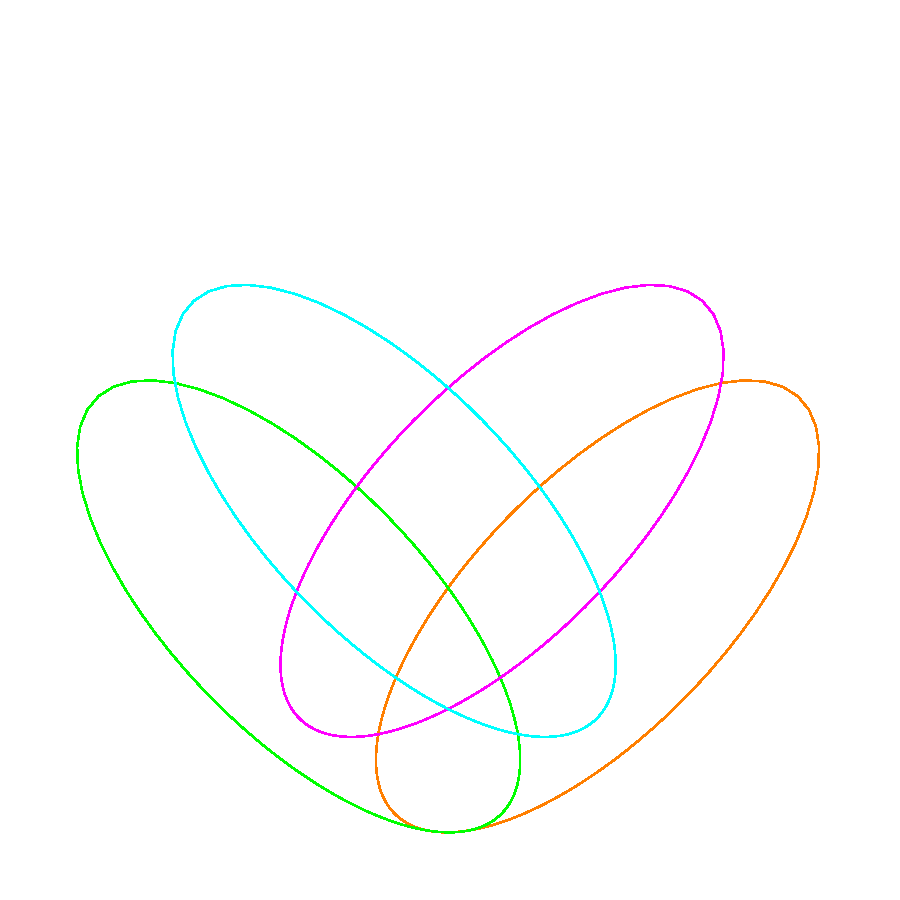
\includegraphics{Vennfig-002}
\end{center}

\newpage
\section{Quick tour}
The Vennerable package provides routines to compute and plot
Venn diagrams, from the classic two- and three-circle diagrams
to diagrams using different shapes and
for up to seven sets. In addition it can plot diagrams in which the
area of each region is proportional to the corresponding number of set items or 
other weights.

Figure \ref{fig:canonical} shows a three-circle Venn diagram of the sort
commonly found. First we construct an object of class \texttt{Venn}:

\begin{Schunk}
\begin{Sinput}
> library(Vennerable)
> Vcombo <- Venn(SetNames = c("Female", 
+     "Visible Minority", "CS Major"), 
+     Weight = c(0, 4148, 409, 604, 
+         543, 67, 183, 146))
\end{Sinput}
\end{Schunk}
This returns an object of (S4) class {\texttt Venn} and 
a call to {\texttt plot} {\texttt plot.Venn} produces the diagram.
\begin{figure}[H]\begin{center}
\begin{Schunk}
\begin{Sinput}
> plot(Vcombo, doWeights = FALSE)
\end{Sinput}
\end{Schunk}
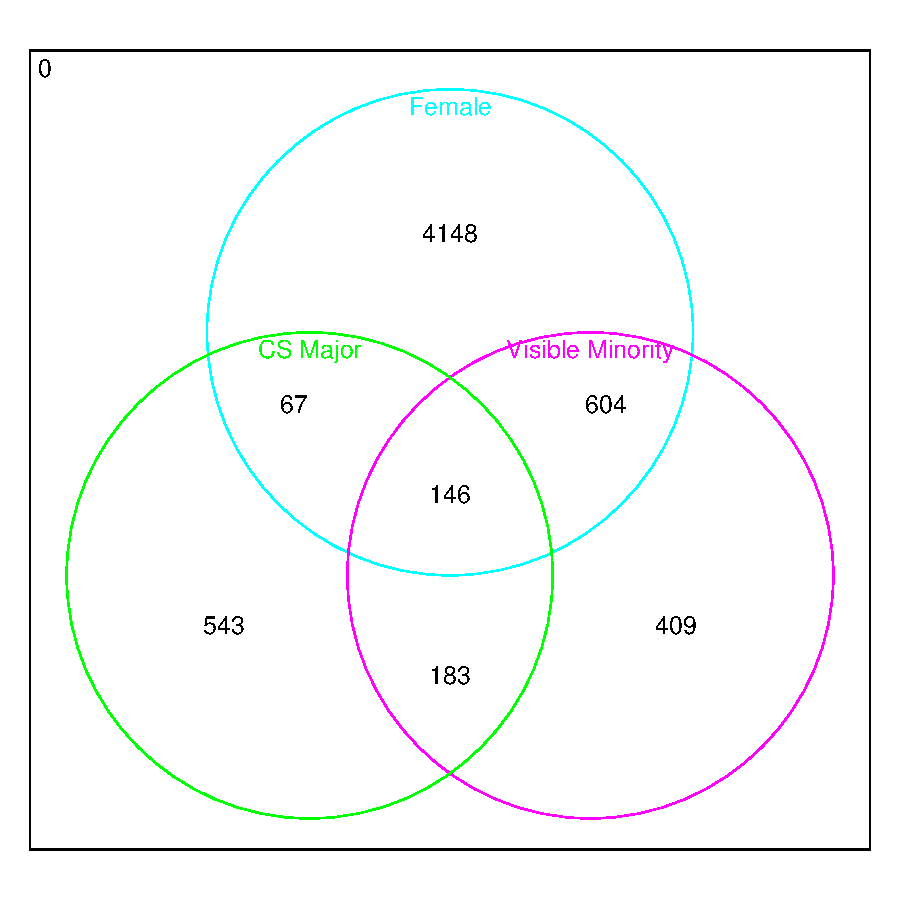
\includegraphics{Vennfig-pVN3}
\caption{A three-circle Venn diagram} 
\label{fig:canonical}
\end{center}\end{figure}

The \texttt{Vennerable} package extends this plot in three ways. First
it allows the use of a variety of other shapes for
the set boundaries, and up to seven different sets.
Secondly it implements a number of published or novel
algorithms for generating diagrams in which the area
of each region is proportional to, for example, the number
of corresponding set elements. Finally it adds a number of
graphical control abilities, including the ability to colour individual
regions separately.

\section{Some loose definitions}
Figure \ref{fig:canonical} illustrates membership of three sets,
in order Female,  Visible Minority, CS Major. 
People who are members of the Visible Minority set are not Female  nor a CS Major
are members of an \emph{intersection subset} with \emph{indicator string} 
\texttt{010}.

Given $n$ sets of elements drawn from a universe,
 there are $2^n$ {intersection subsets}. Each of these is 
a subset of the universe and there
is one corresponding to each of  the binary strings of length $n$.
If one of these indicator strings has a 1 in the $i$-th position, all of members of the 
corresponding intersection subset must be members of the $i$-th set. Depending on the application, the 
universe of elements from which members of the sets are drawn 
may be important. 
Elements in intersection set \texttt{00\ldots}, which are in 
the universe but not in any known set, are called \emph{dark matter},
and we tend to display these differently.

A diagram which produces a visualisation of each of the sets
as a connected curve in the plane whose regions of intersection
are connected and correspond to each of the $2^n$ intersection subsets
is an \emph{unweighted Venn diagram}.
Weights can be assigned to each of the intersections,
most naturally being proportional to the number of elements each one contains.
\emph{Weighted Venn diagrams} have the same topology as unweighted ones, but 
(attempt to) make the area of each region proportional to the weights. 
This may not be possible, if any of the weights are zero for example, or because 
of the geometric constraints of the diagram. Venn diagrams based on 3 circles
are unable in general to represent even nonzero weights exactly, and cannot be constructed
at all for $n>3$.

Diagrams in which only those intersections with non-zero weight appear are \emph{Euler diagrams},
and diagrams which go further and make the area of every intersection proportional to its weight are weighted Euler diagrams.
For more details and rather more rigour see first the online review of Ruskey and Weston\cite{ruskeyweston:2005}.


\section{Unweighted Venn diagrams}

For a running example, we use sets named after months,
whose elements are the letters of their names.
\begin{Schunk}
\begin{Sinput}
> setList <- strsplit(month.name, split = "")
> names(setList) <- month.name
> VN3 <- VennFromSets(setList[1:3])
> V2 <- VN3[, c("January", "February"), 
+     ]
\end{Sinput}
\end{Schunk}
More details on the construction of  {\texttt Venn} objects is given in Section \ref{sec:venn}.


\subsection{Unweighted 2-set Venn diagrams}

The geometry of the diagram is controlled with the \texttt{type} argument
which, for two sets, can be \texttt{type=circles} or \texttt{type=squares}.
The full code for producing the Figure
can be found by consulting the source of this vignette \texttt{Venn.Rnw}
in the \texttt{inst/doc} subdirectory of the \texttt{Vennerable} package.
 
\begin{figure}[H]\begin{center}

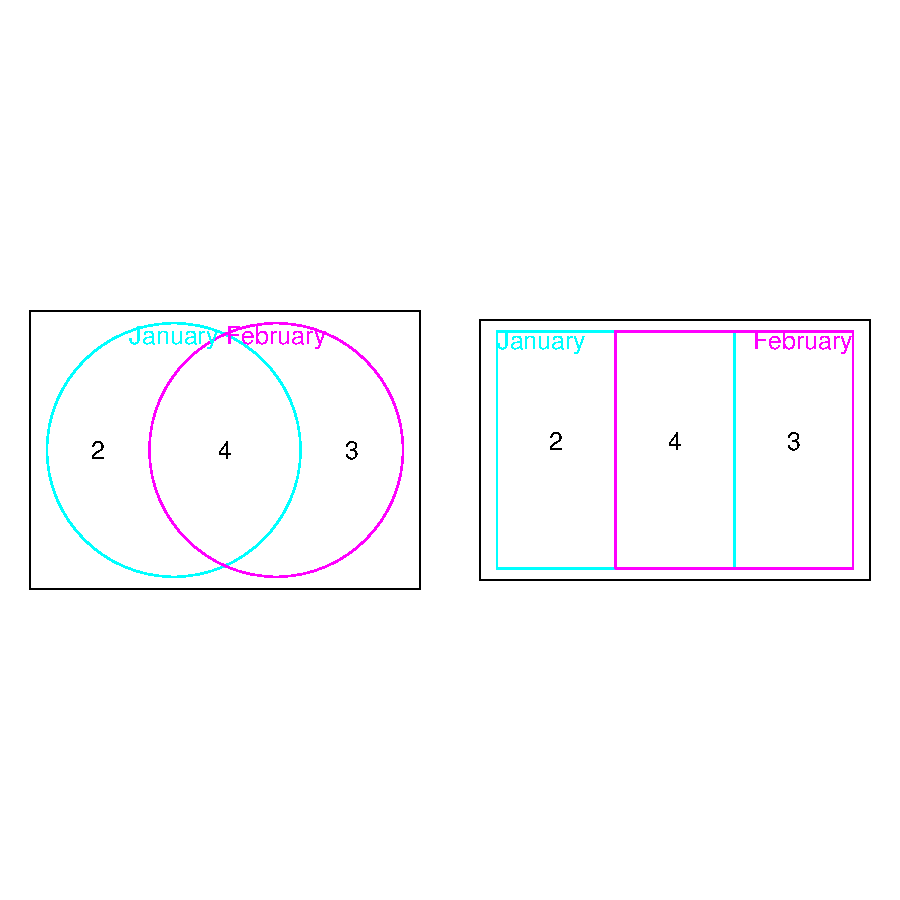
\includegraphics{Vennfig-pv2uwwww}
\caption{Unweighted 2-set Venn diagrams with \texttt{type=circles} or \texttt{type=squares}}
\end{center}\end{figure}

\newpage
\subsection{Unweighted 3-set Venn diagrams}
For three sets, the \texttt{type} argument
can be \texttt{circles}, \texttt{squares}, 
\texttt{ChowRuskey}, \texttt{triangles} or \texttt{AWFE}.
The Chow-Ruskey plot is from \cite{chowruskey:2005}.
The AWFE plot is a somewhat ugly implementation of the elegant
ideas of  \cite{edwards:2004}. 
The triangles plot is new as far as I know.


% TODO triangles and AWFE comment
\begin{figure}[H]\begin{center}
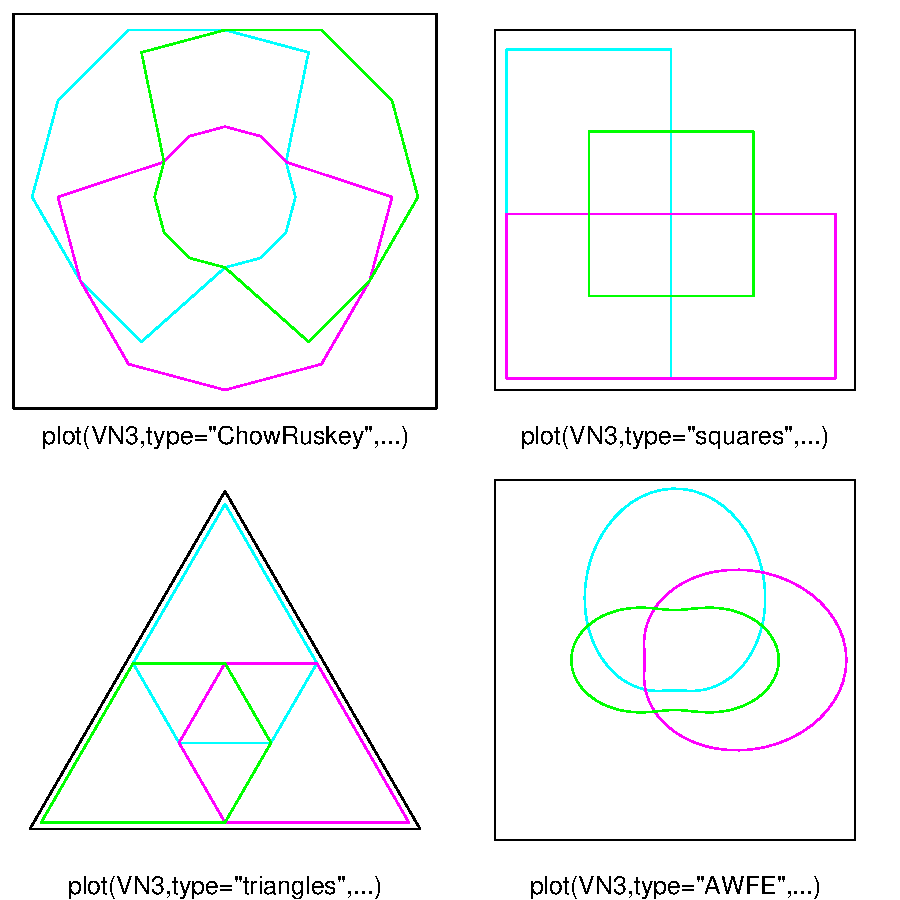
\includegraphics{Vennfig-pv3uwww}
\end{center}\end{figure}
\newpage
\subsection{Unweighted 4-set Venn diagrams}
For four sets, the \texttt{type} argument
can be  \texttt{ChowRuskey}, \texttt{AWFE},\texttt{squares} or \texttt{ellipses}.

The squares plot is said by Edwards \cite{edwards:2004} to have
been introduced by Lewis Carroll \cite{carroll:1896}.
The ellipse plot was suggested by Venn \cite{venn:1880}.


\begin{figure}[H]\begin{center}
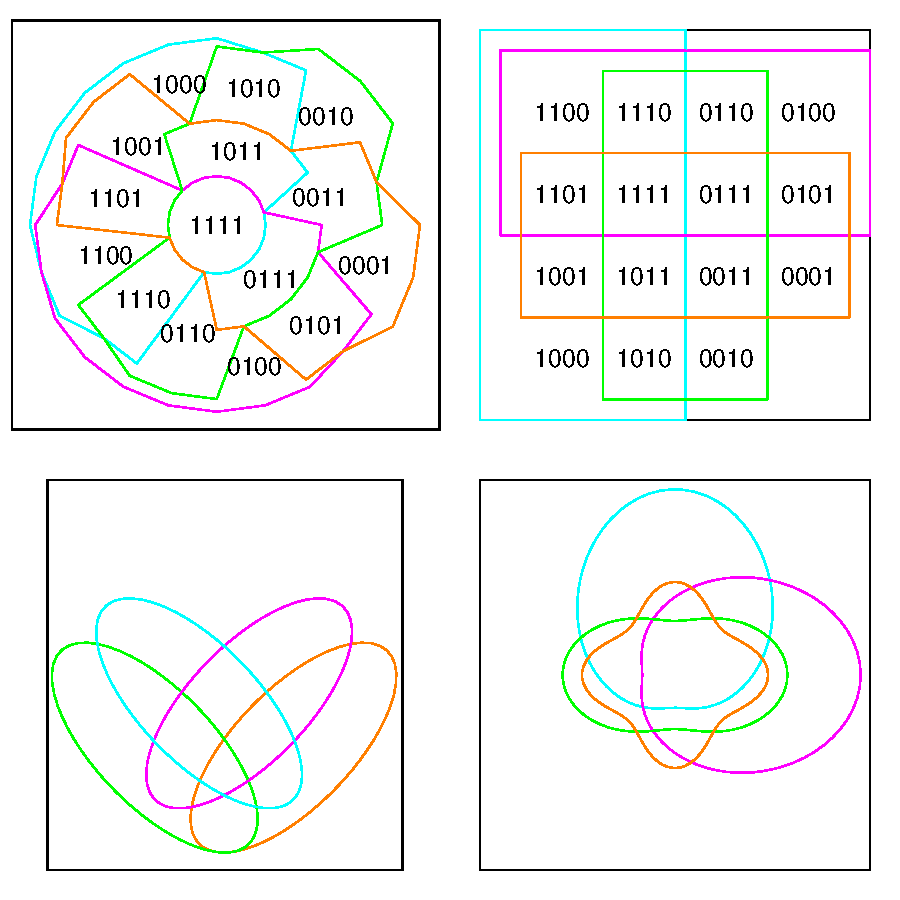
\includegraphics{Vennfig-pV4uw}
\caption{Venn diagrams on four sets.
}
\end{center}\end{figure}

A number of variants on the \texttt{squares} type are implemented,
but require finer control over the diagram creation process.
\begin{Schunk}
\begin{Sinput}
> doans <- function(V4, s, likeSquares) {
+     S4 <- compute.S4(V4, s = s, likeSquares = likeSquares)
+     anlay <- grid.layout(2, 1, heights = unit(c(1, 
+         1), c("null", "lines")))
+     pushViewport(viewport(layout = anlay))
+     txt <- ""
+     pushViewport(viewport(layout.pos.row = 2))
+     grid.text(label = txt)
+     popViewport()
+     pushViewport(viewport(layout.pos.row = 1))
+     CreateViewport(S4)
+     PlotSetBoundaries(S4, gp = gpar(lwd = 4:1, 
+         col = trellis.par.get("superpose.symbol")$col))
+     UpViewports()
+     popViewport()
+     popViewport()
+ }
\end{Sinput}
\end{Schunk}
For more details on this see the help pages and \ref{sec:graphics}.

\begin{figure}[H]\begin{center}
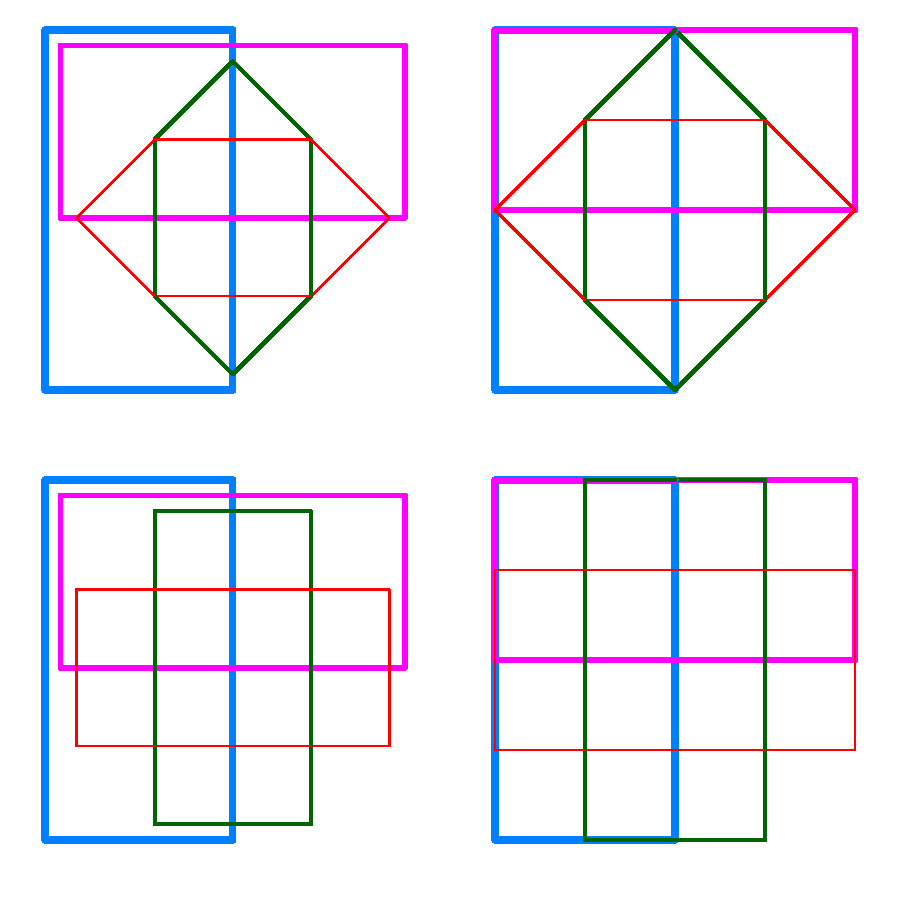
\includegraphics{Vennfig-S4fig}
\caption{Four variants on the four-squares}
\end{center}\end{figure}


\clearpage
\subsection{Unweighted Venn diagrams on more than four sets}

The package implements a (somewhat ugly) variant of the Edwards construction
for Venn diagrams on an arbitrary number of sets $n$. The currently implemented algorithm is rather 
inefficient and is only feasible to compute quickly for $n<7$. 

\begin{figure}[H]\begin{center}
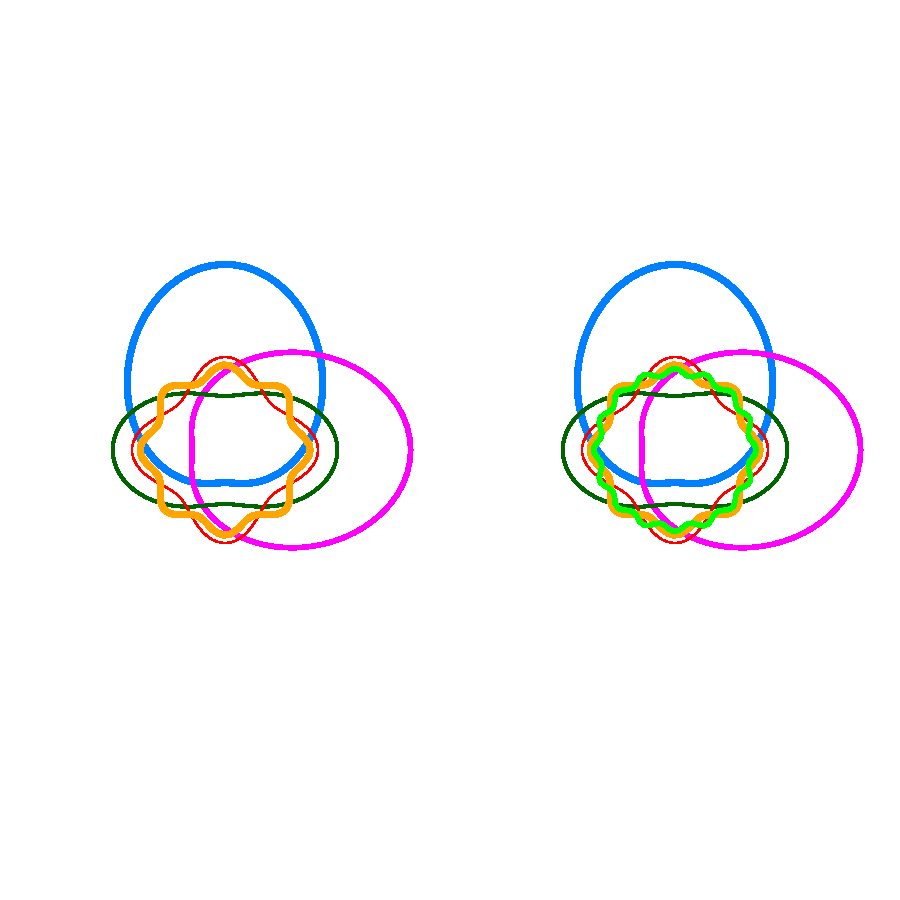
\includegraphics{Vennfig-S47fig}
\caption{Edwards constructions for five and six sets}
\end{center}\end{figure}











\newpage
%########################################################
\section{Weighted Venn diagrams}
% TODO some discussion on the point
In this section we show Venn diagrams with weights
which are (with the possible exception of dark matter) all nonzero.



\subsection{Weighted 2-set Venn diagrams for 2 Sets}
\subsubsection{Circles}
It is always possible to get an exactly area-weighted solution for two circles 
as shown in Figure \ref{fig:pv2b2}.


\begin{figure}[H]
  \begin{center}
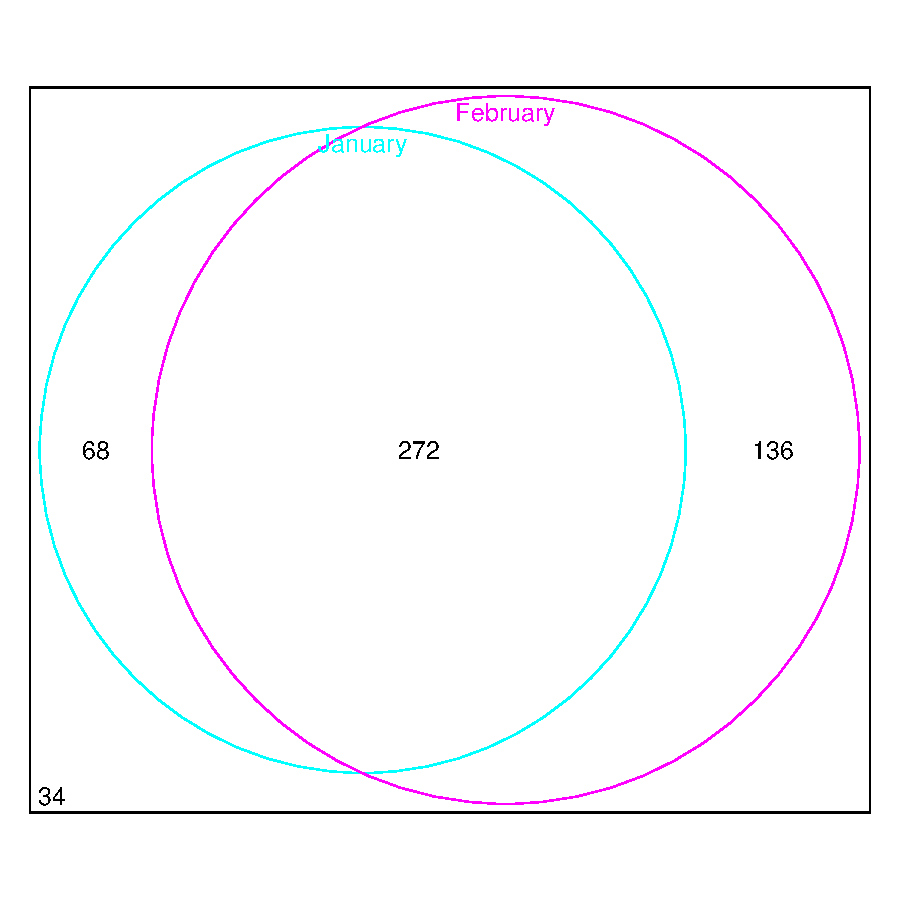
\includegraphics{Vennfig-pv2b2}
\caption{Weighted 2d Venn}
\label{fig:pv2b2}
\end{center}\end{figure}




\subsubsection{Squares}
As for circles, square Venn and Euler diagrams on two sets 
can be simply constructed.
\begin{figure}[H]
  \begin{center}
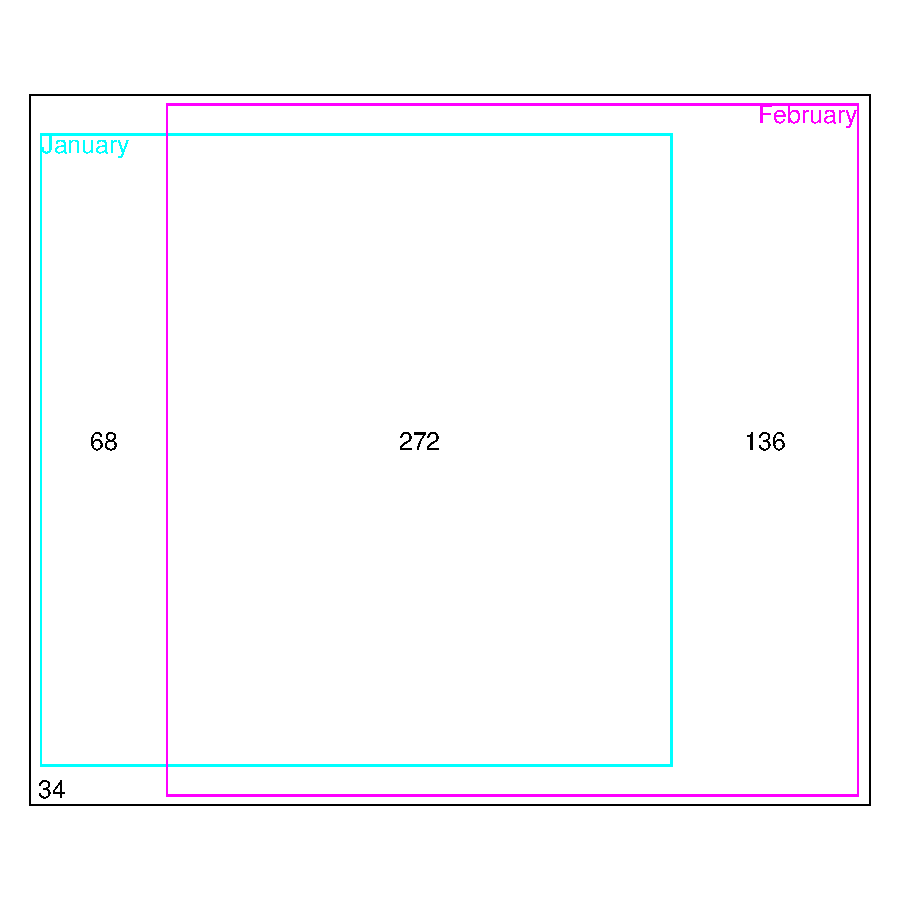
\includegraphics{Vennfig-sqpv2b}
\caption{Weighted 2d Venn squares}
\end{center}\end{figure}

\newpage
\subsection{Weighted 3-set Venn diagrams}

\subsubsection{Circles}
There is no general way of creating area-proportional
3-circle diagrams. The package makes an attempt
to produce approximate ones.
\begin{figure}[H]
  \begin{center}
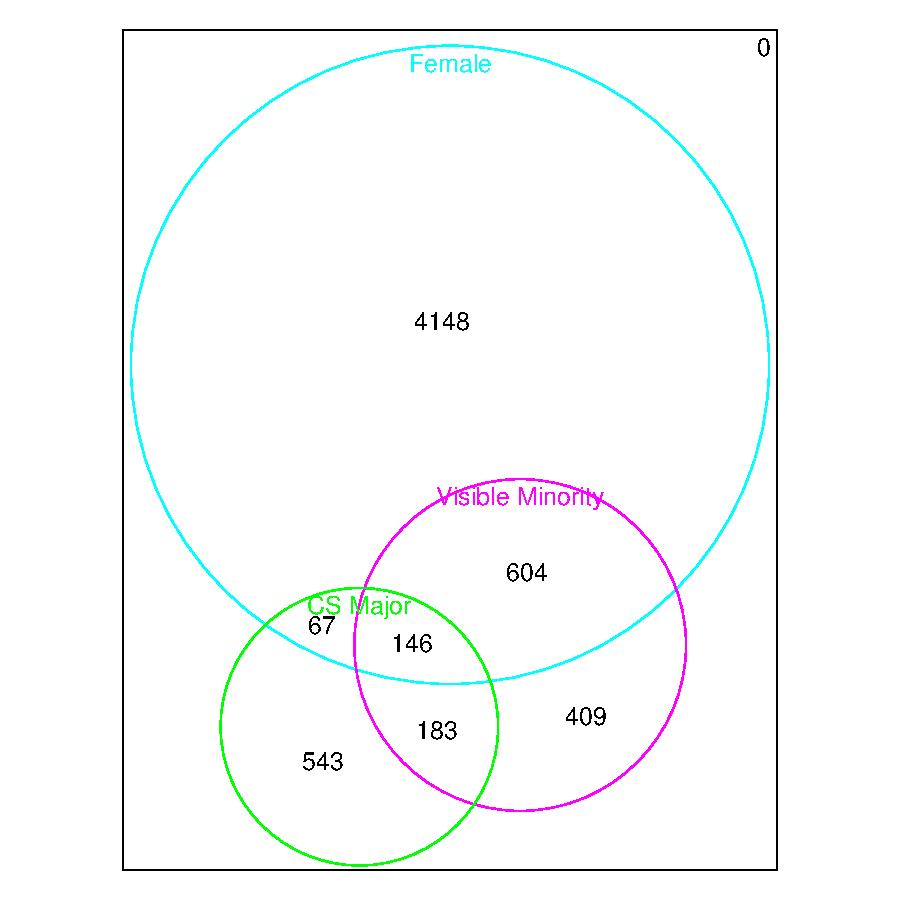
\includegraphics{Vennfig-ccomboutransp}
  \caption{ 3D Venn diagram }
  \end{center}
\end{figure}
The algorithm used is to compute the individual circles to have the exact area necessary
for proportionality, and then compute each of the three pairwise distances
between centres necessary for the correct pairwise areas. If these distances do not satisfy the triangle inequality
the largest is reduced until they do. Then the circles are arranged with their centres
separated by these (possibly modified) distances.



\newpage

\subsubsection{Squares}
This is a version of the algorithm suggested by \citet{chowruskey:2003}.

\begin{figure}[H]\begin{center}
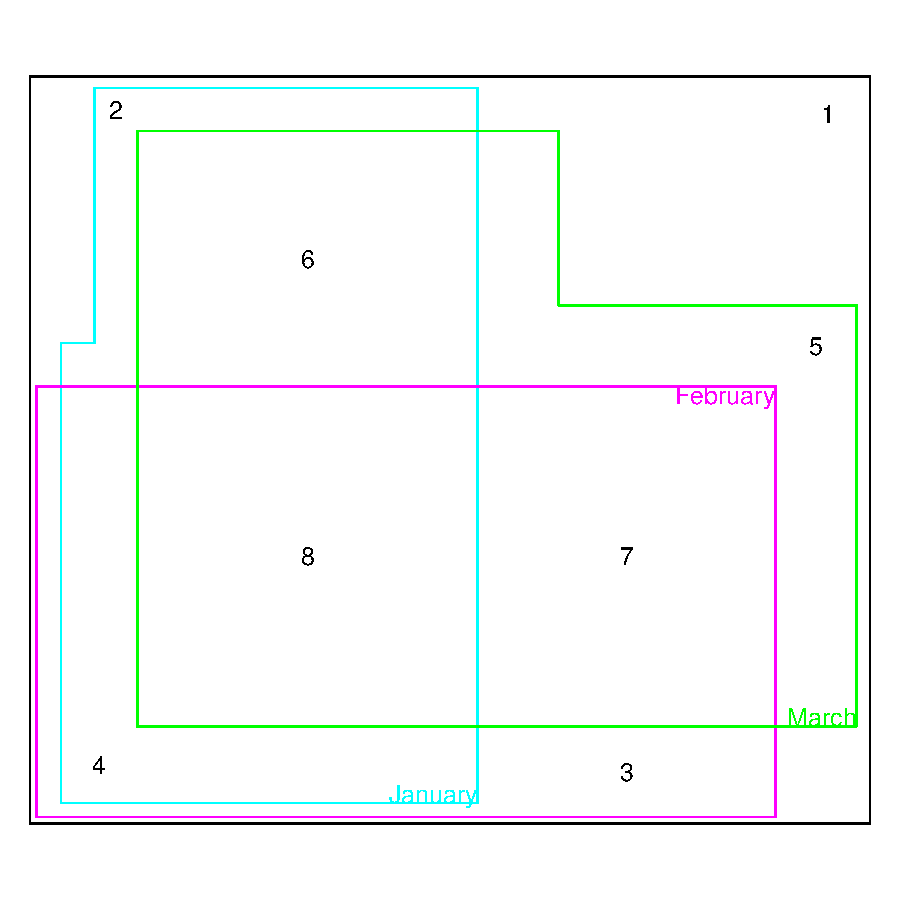
\includegraphics{Vennfig-S3ccpdemo}
\caption{Weighted 3-set Venn diagram based on the algorithm of \citet{chowruskey:2003}}
\end{center}\end{figure}


\newpage

\subsubsection{Triangles}
The triangular Venn diagram on 3-sets lends itself nicely to
an area-proportional drawing under some contraints on the weights.
These constraints are that
\begin{eqnarray}
4 w_a w_b w_c  < (1 -  (w_a+w_b+w_c))^2
\end{eqnarray}
must hold for both of the sets of numbers
\begin{eqnarray}
w_a &=& w_{100}
\\
w_b &=& w_{010}
\\
w_c &=& w_{001}
\end{eqnarray}
and
\begin{eqnarray}
w_a &=& w_{101}/W
\\
w_b &=& w_{011}/W
\\
w_c &=& w_{011}/W
\end{eqnarray}
where $w_s$ is the normalised weight of the set with indicator string $s$ and
$W=w_{101}+w_{011}+w_{011}+w_{111}=1-(w_{100}+w_{010}+w_{001})$.


\begin{figure}[H]\begin{center}
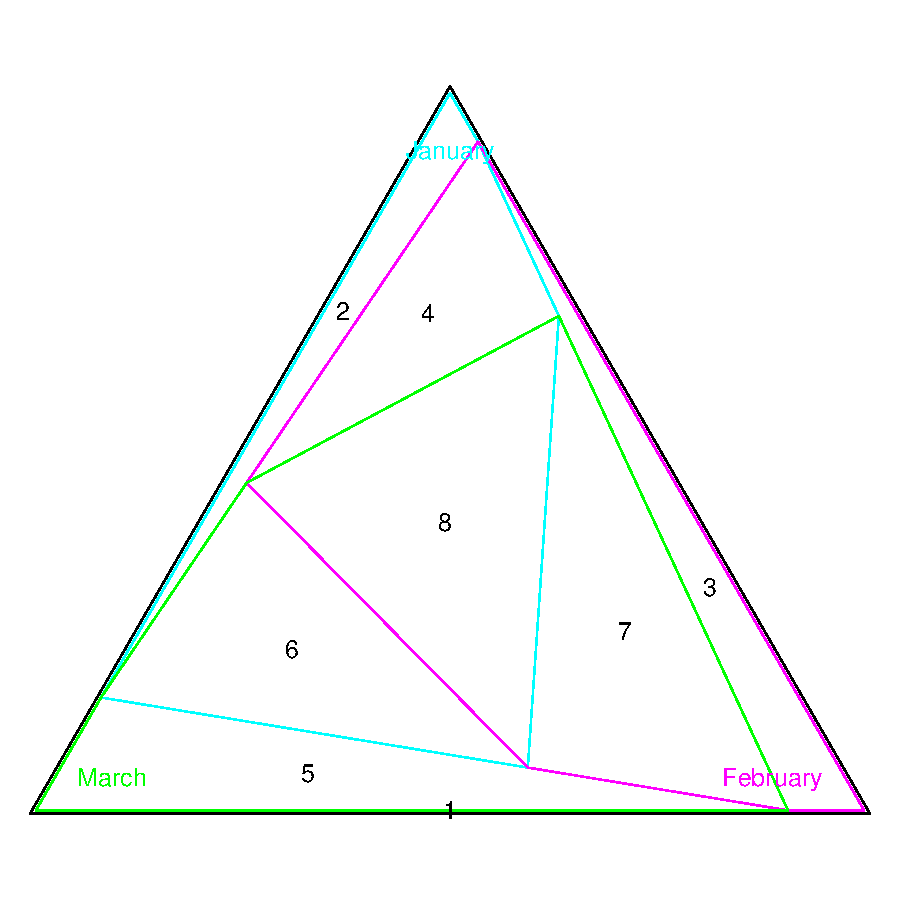
\includegraphics{Vennfig-plotT3}
\caption{Triangular Venn with external universe}
\end{center}
\end{figure}

\newpage

\subsection{Chow-Ruskey diagrams for 3 or more sets}
The general Chow-Ruskey algorithm  \cite{chowruskey:2005} can be implemented
in principle for an arbitrary number of sets provided
the weight of the common intersection is nonzero.

\begin{figure}[H]\begin{center}
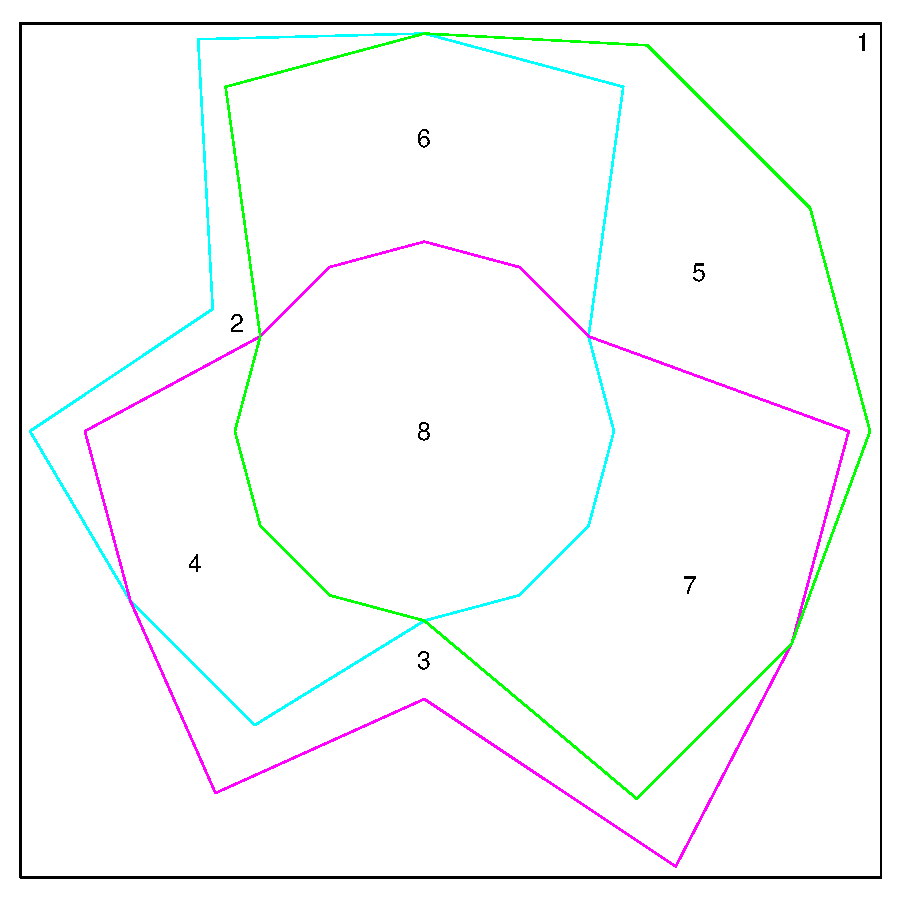
\includegraphics{Vennfig-plotCR3}
\caption{Chow-Ruskey weighted 3-set diagram}
\end{center}
\end{figure}

\begin{figure}[H]\begin{center}
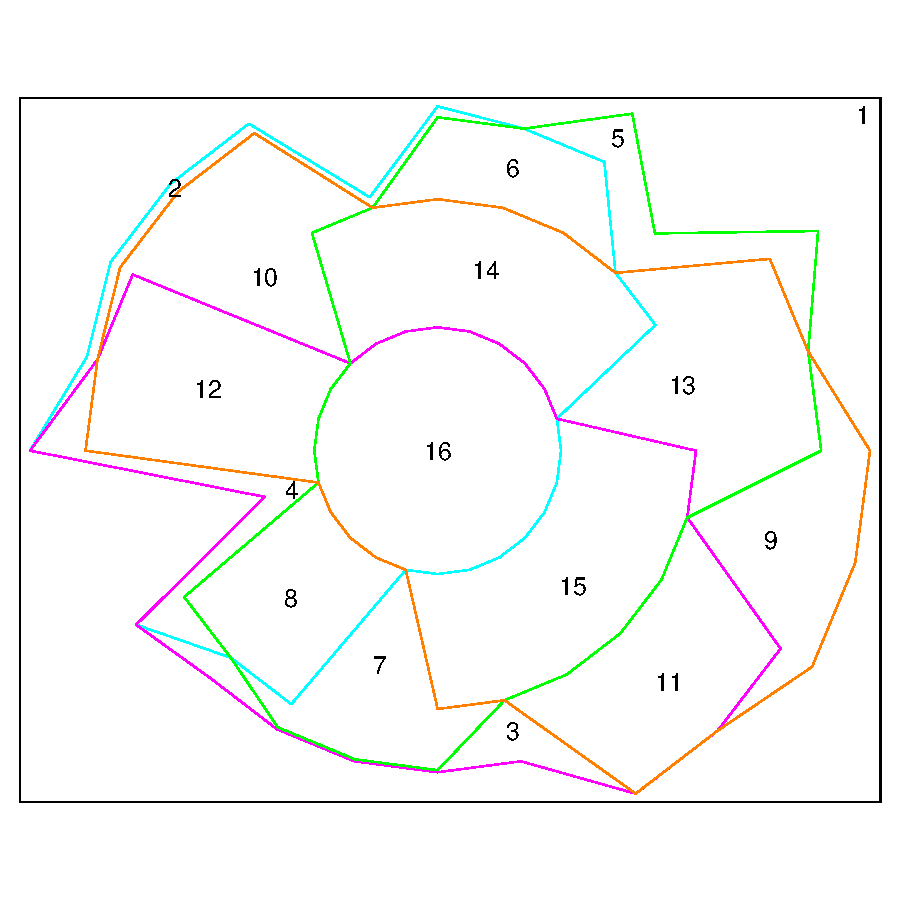
\includegraphics{Vennfig-plotCR4}
\caption{Chow-Ruskey weighted 4-set diagram}
\end{center}
\end{figure}

\newpage
%########################################################
\section{Euler diagrams}

As we have seen, for some geometries it is not possible
to enforce exact area-proportionality when requested by the \texttt{doWeight=TRUE} argument,
and an attempt is made to produce an approximately area-proportional diagram. In
particular, regions whose weight is zero may appear with nonzero areas.
 A separate 
requirement which is desirable in some cases, especially high dimensional ones,
is to ensure that regions of zero weight are not displayed at all, producing an \emph{Euler diagram}. 
This can be achieved, for some geometries, by use of the \texttt{doEuler=TRUE} argument.
These two flags can interact in weird and uncomfortable ways depending on
exactly which intersection weights are zero.

\subsection{2-set Euler diagrams}

\subsubsection{Circles}


\begin{figure}[H]\begin{center}
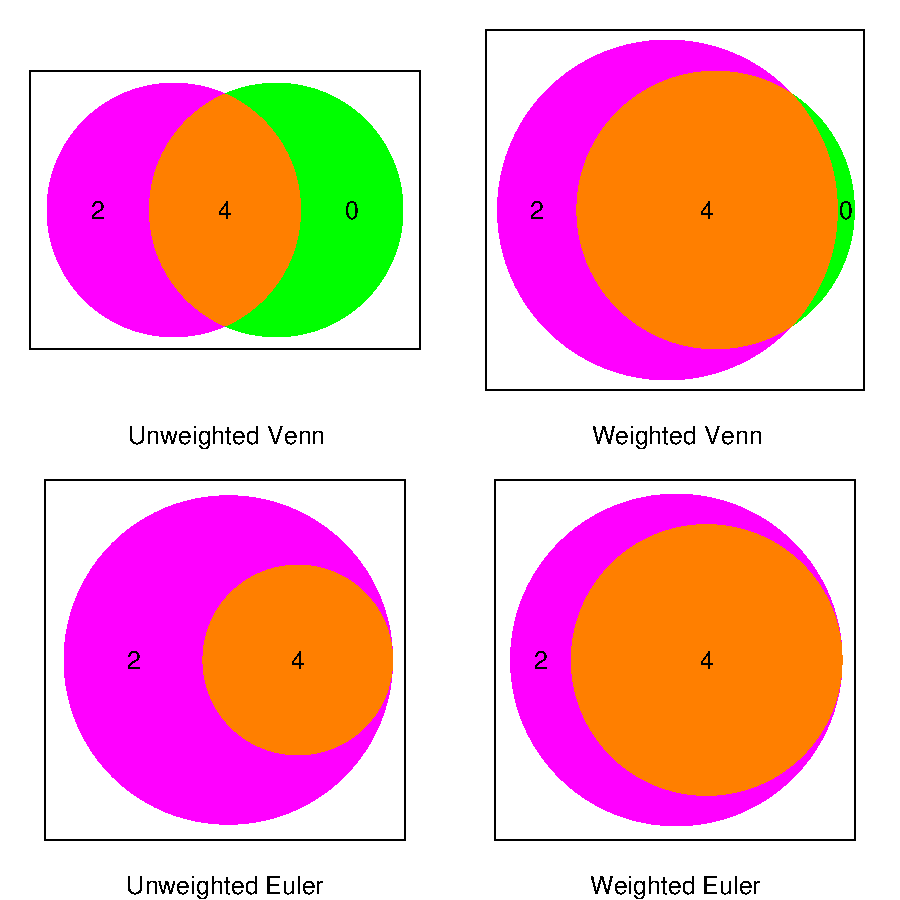
\includegraphics{Vennfig-p2threef01}
\caption{Effect of the Euler and \texttt{doWeights} flags.}
\end{center}\end{figure}


\begin{figure}[H]\begin{center}
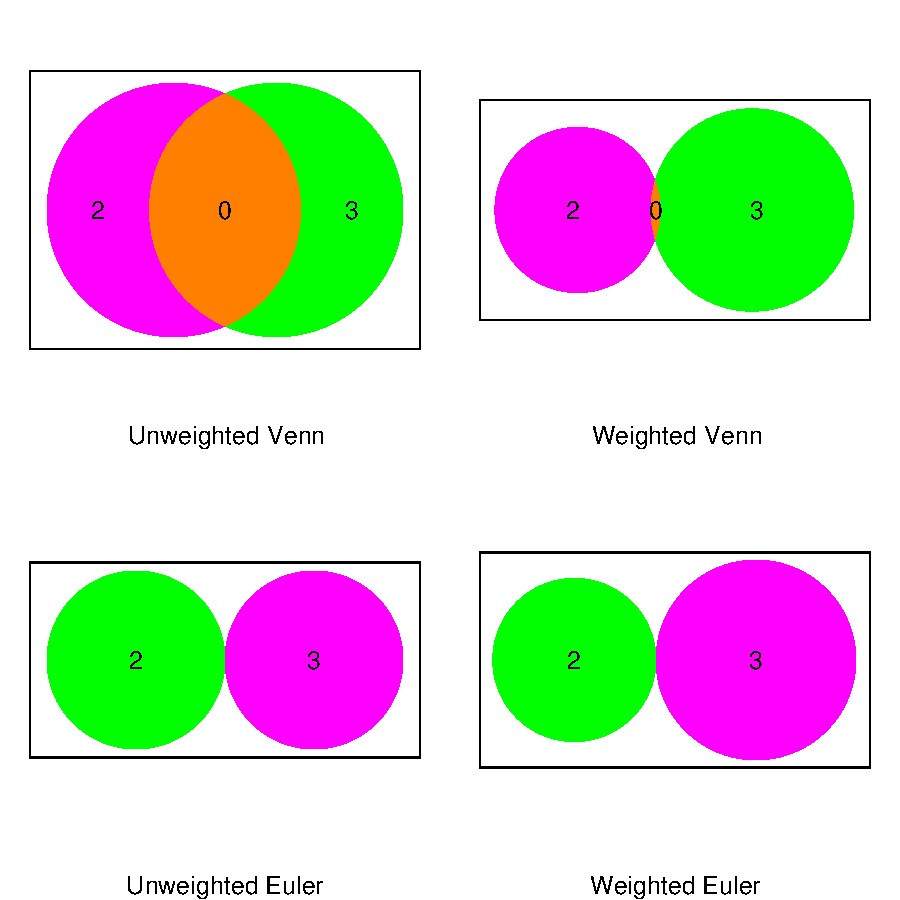
\includegraphics{Vennfig-p2no11threef}
\caption{As before for a set of weights with different zeroes}
\end{center}\end{figure}

\subsubsection{Squares}
As for circles, the idea of a weighted Venn diagram when some of the weights
are zero doesn't make much sense in theory but might be useful for making visual 
points. 
\begin{figure}[H]\begin{center}
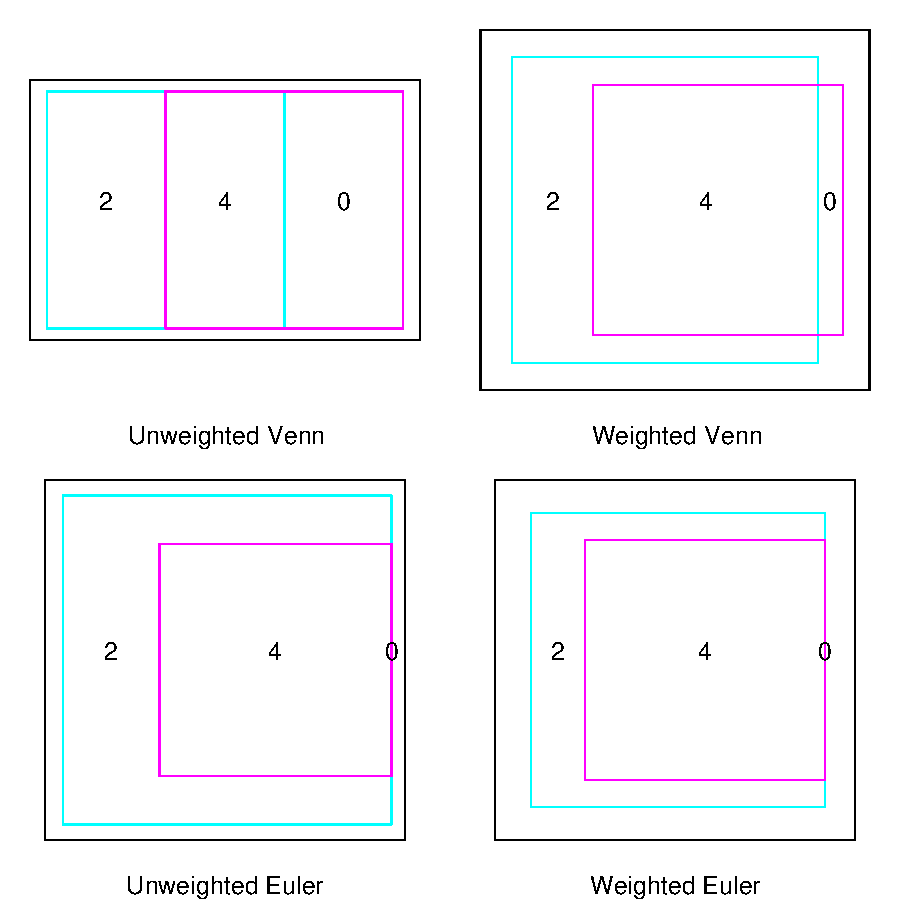
\includegraphics{Vennfig-p2s01threef}
\end{center}\end{figure}


\begin{figure}[H]\begin{center}
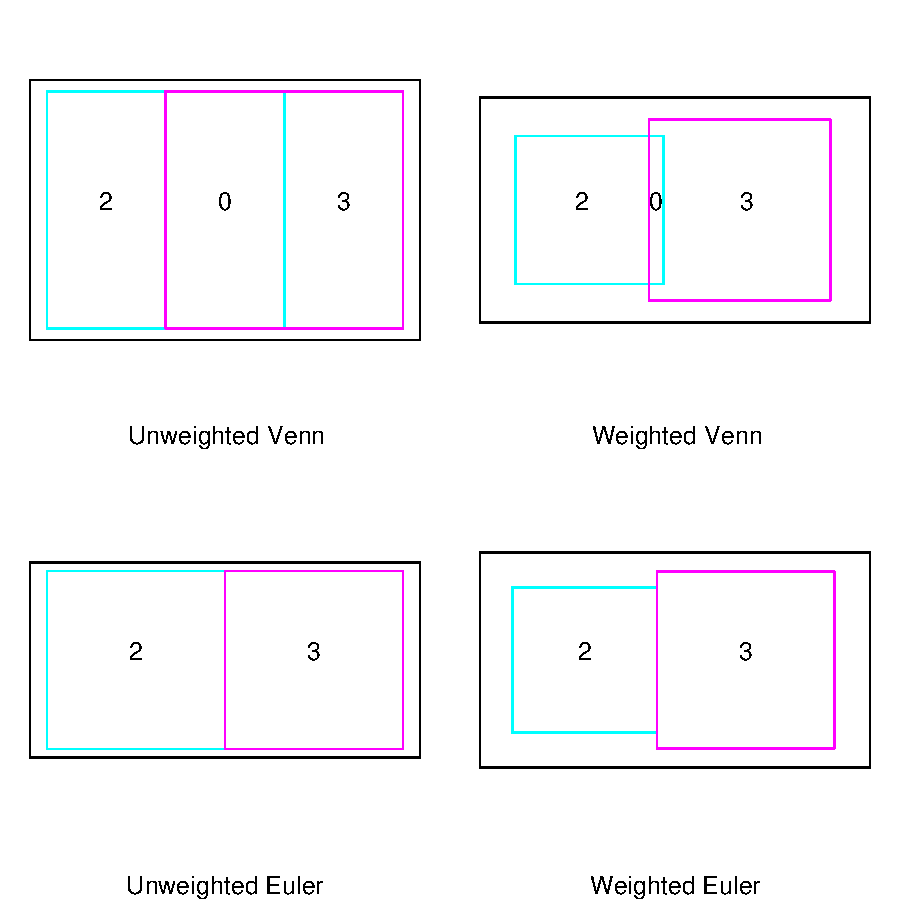
\includegraphics{Vennfig-p2sthreef}
\end{center}\end{figure}

\newpage
\subsection{3-set Euler diagrams}

\subsubsection{Circles}
There is currently no effect of setting \texttt{doEuler=TRUE} for three circles,
but the \texttt{doWeights=TRUE} flag does an approximate job. There are about
 40 distinct ways in which intersection regions can have zeroes can occur,
but here are some examples.




\begin{figure}[H]\begin{center}
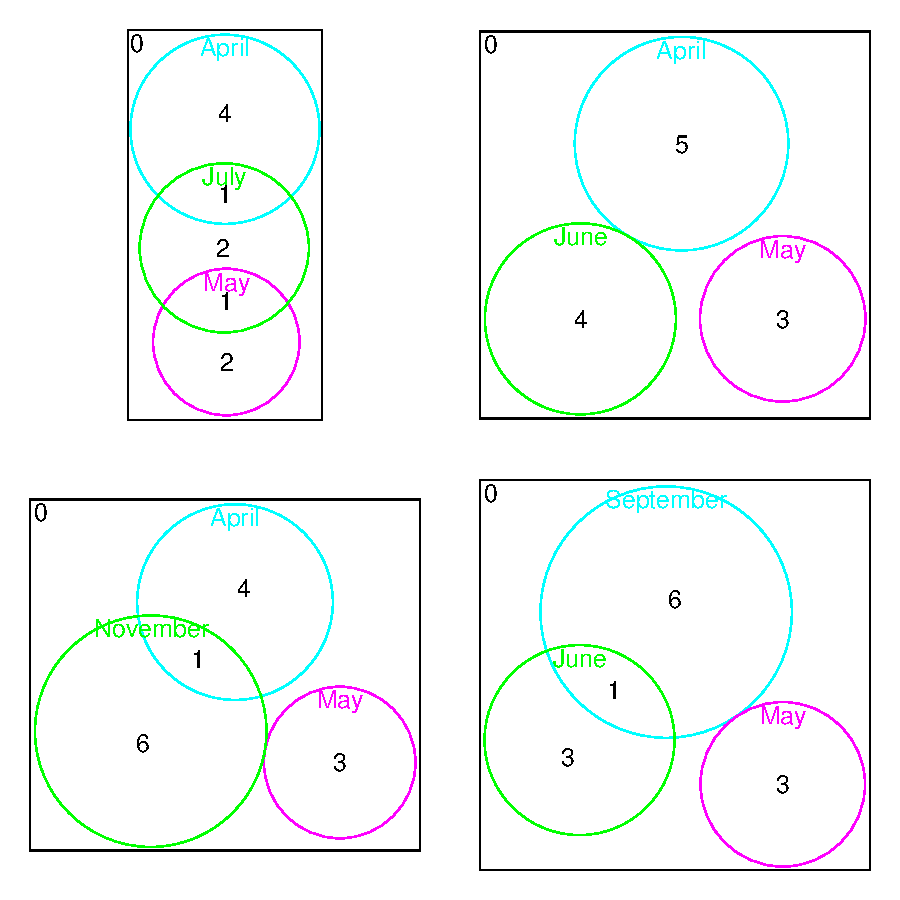
\includegraphics{Vennfig-pv3wempty}
\caption{Weighted 3d Venn  empty intersections}
\end{center}\end{figure}


\clearpage
\subsubsection{Triangles}


The \texttt{doEuler} flag has no effect for triangles; all
the weighted diagrams produced are Euler diagrams.
\begin{figure}[H]\begin{center}
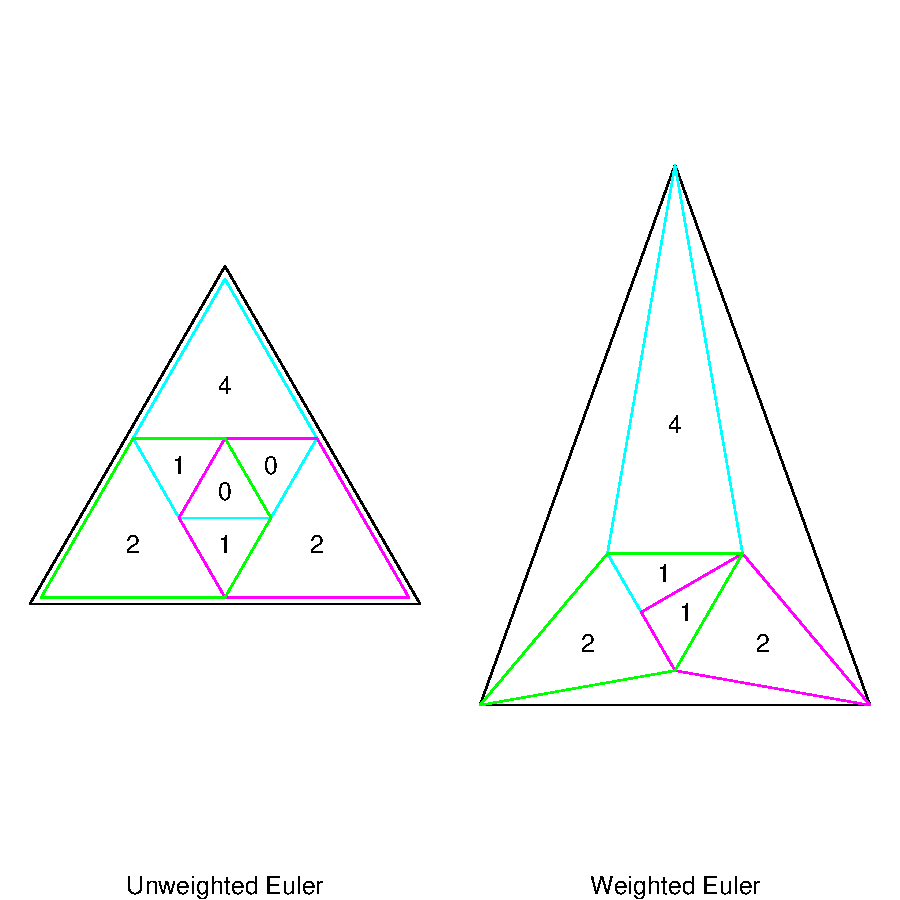
\includegraphics{Vennfig-pv3wempty1t}
\caption{3d Venn triangular with two zero weights}
\end{center}\end{figure}

\begin{figure}[H]\begin{center}
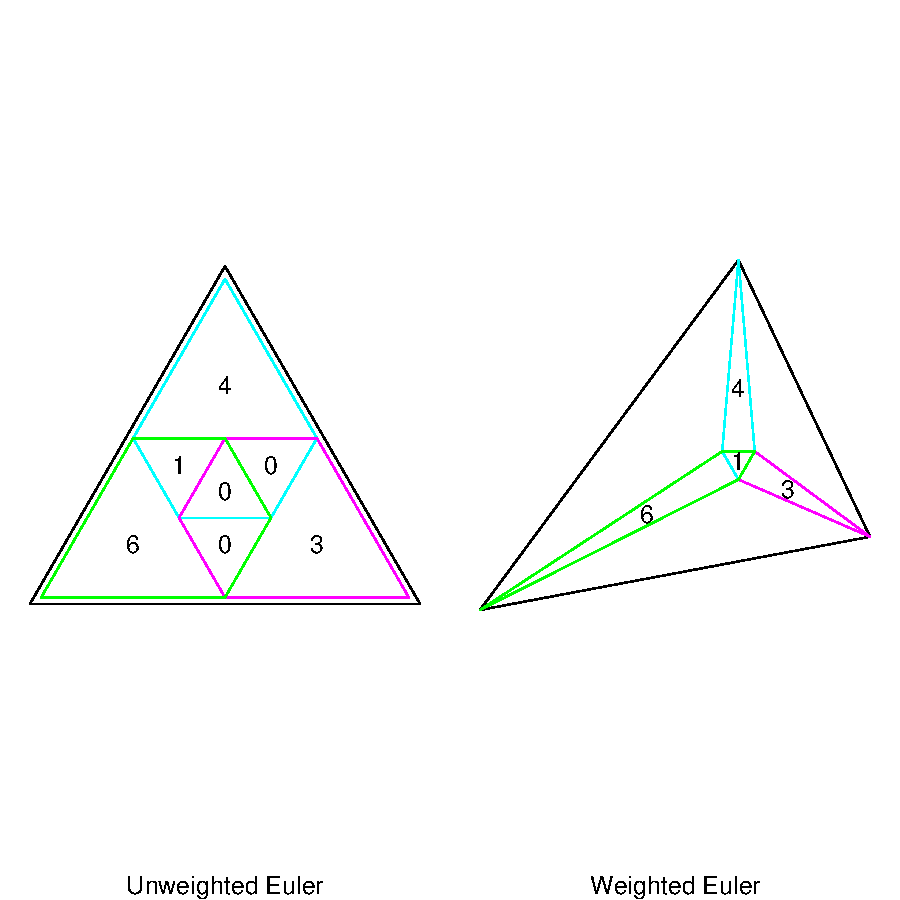
\includegraphics{Vennfig-pv3wempty2t}
\caption{3d Venn triangular witht three zero weights}
\end{center}\end{figure}

\subsection{4-set Euler diagrams}
\subsubsection{Chow-Ruskey diagrams}


The \texttt{doEuler} flag has no effect for Chow-Ruskey; all
the weighted diagrams produced are Euler diagrams.

\begin{figure}[H]\begin{center}
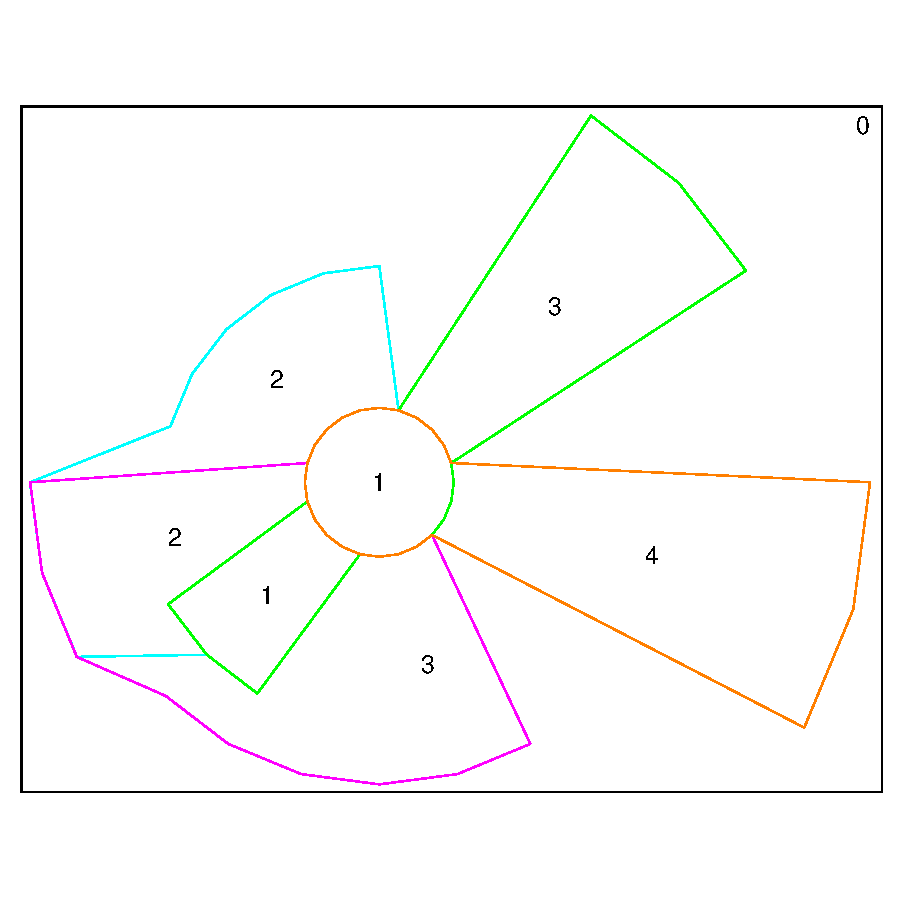
\includegraphics{Vennfig-CR4fig}
\caption{Chow-Ruskey diagram with some zero weights}
\end{center}\end{figure}

%########################################################
\clearpage
\newpage
\section{Constructing {\texttt Venn} objects}
\label{sec:venn}
% TODO define weights properly via named vector
A {\texttt Venn} object has weights associated with each intersection; by default
the weight is the number of elements in the intersection.
{\texttt Venn} objects can be constructed with arbitrary weights:
\begin{Schunk}
\begin{Sinput}
> V3 <- Venn(SetNames = month.name[1:3])
> Weights(V3) <- c(0, 81, 81, 9, 81, 
+     9, 9, 1)
\end{Sinput}
\end{Schunk}

The resulting object has a number of functions defined on it:
\begin{Schunk}
\begin{Sinput}
> SetNames(V3)
\end{Sinput}
\begin{Soutput}
[1] "January"  "February" "March"   
\end{Soutput}
\begin{Sinput}
> Weights(V3)
\end{Sinput}
\begin{Soutput}
000 100 010 110 001 101 011 111 
  0  81  81   9  81   9   9   1 
\end{Soutput}
\begin{Sinput}
> NumberOfSets(V3)
\end{Sinput}
\begin{Soutput}
[1] 3
\end{Soutput}
\begin{Sinput}
> Indicator(V3)
\end{Sinput}
\begin{Soutput}
     January February March
[1,]       0        0     0
[2,]       1        0     0
[3,]       0        1     0
[4,]       1        1     0
[5,]       0        0     1
[6,]       1        0     1
[7,]       0        1     1
[8,]       1        1     1
\end{Soutput}
\end{Schunk}



\subsection{Diagrams for 2 Sets}

Venn objects can be restricted to a smaller number of Sets.
\begin{Schunk}
\begin{Sinput}
> V2 <- VN3[, 1:2, ]
> V2 <- VN3[, c("January", "February"), 
+     ]
> Weights(V2)
\end{Sinput}
\begin{Soutput}
00 10 01 11 
 3  2  3  4 
\end{Soutput}
\end{Schunk}
Note how the weights of the intersections have been updated.


\section{Graphics control}
TODO rather more here
\label{sec:graphics}
\subsection{Annotation}
There are  number of annotation options

\begin{figure}[H]
  \begin{center}
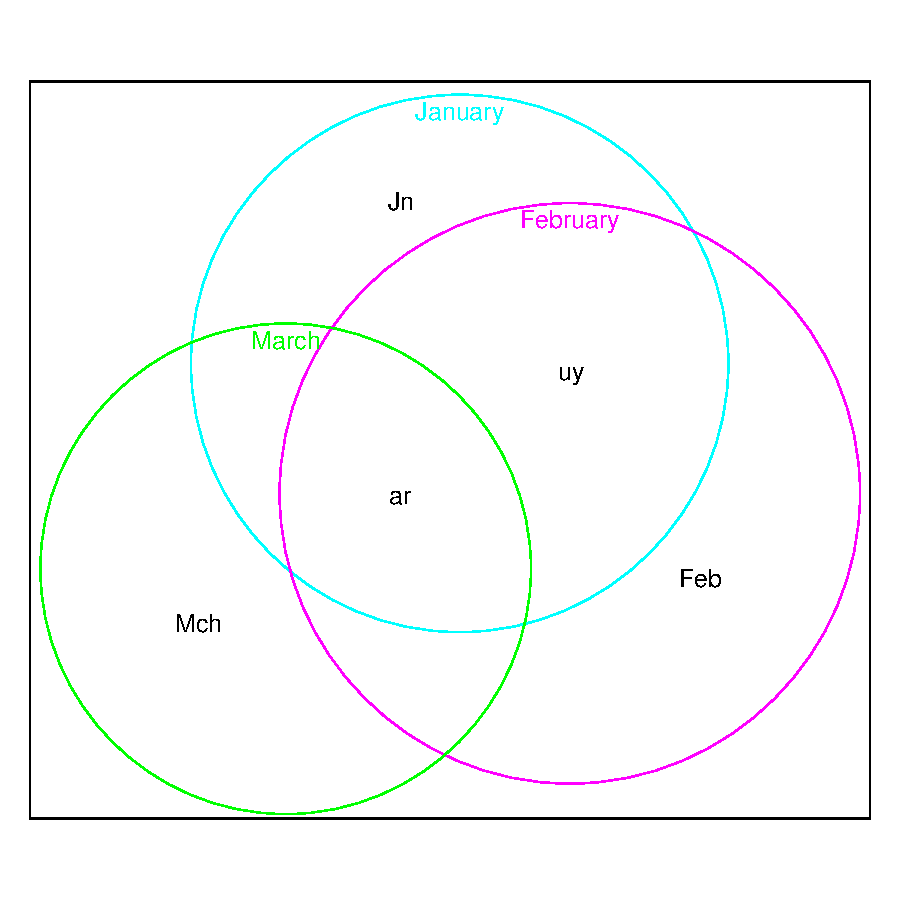
\includegraphics{Vennfig-pv3winn}
\caption{Approximate weighted 3d Venn showing element set membership}
\end{center}\end{figure}


\subsection{Filled sets and transparency}

Some geometries allow for a separate colour specification for 
each intersection region. Even for those that don't, a similar effect
can be obtained using transparent fill colours, but this is only implemented
for some graphics devices. In particular it cannot be seen within R under Windows,
but it is implemented with PDF devices with version number greater than 1.4.


\begin{figure}[H]
  \begin{center}
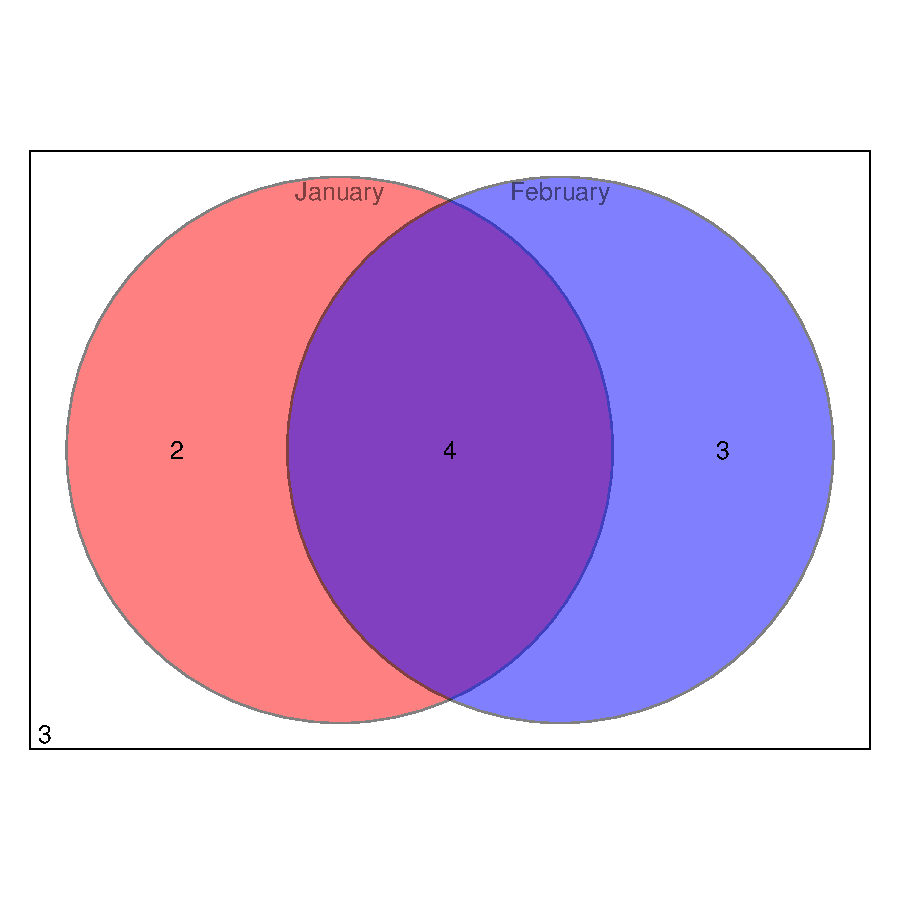
\includegraphics{Vennfig-p2utransp}
  \caption{ 2D Venn diagram with transparency}
  \end{center}
\end{figure}


\begin{figure}[H]
  \begin{center}
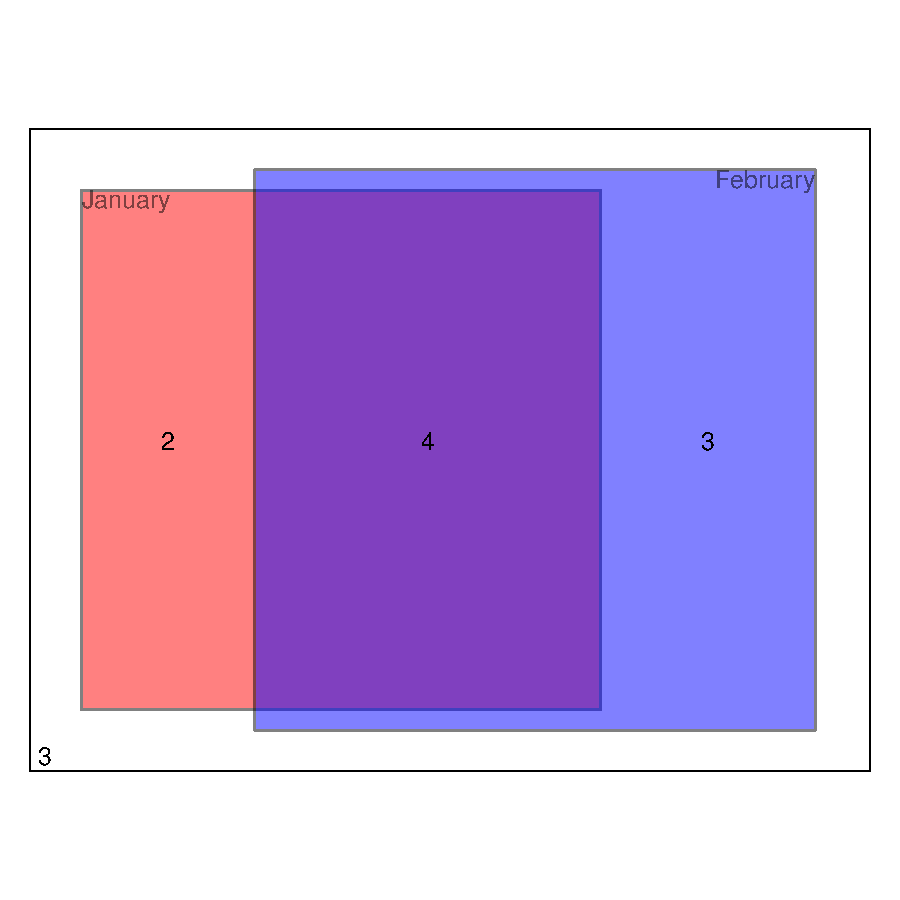
\includegraphics{Vennfig-sq2utransp}
  \caption{ 2D square Venn diagram with transparency}
  \end{center}
\end{figure}

\begin{figure}[H]
  \begin{center}
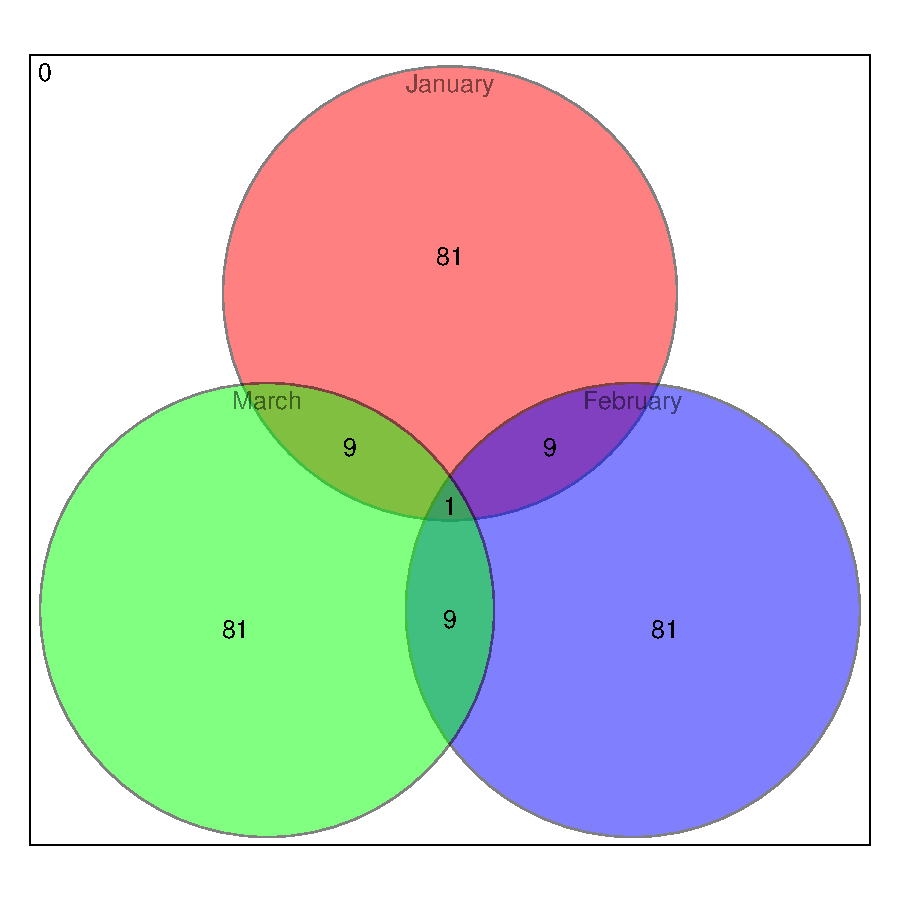
\includegraphics{Vennfig-p3utransp}
  \caption{ 3D Venn diagram with transparency}
  \end{center}
\end{figure}




\section{This document}

\begin{tabular}{|l|l|}
\hline
Author & Jonathan Swinton
\\
CVS id of this document & ${}$Id: Venn.Rnw,v 1.24 2007/04/23 22:10:13 js229 Exp ${}$.
\\
Generated on & \today
\\
R version & 
R version 2.6.0 Under development (unstable) (2007-06-11 r41912)\\
\hline
\end{tabular}

\bibliographystyle{plain}
\bibliography{Venn}

\end{document}
